\documentclass[10pt]{beamer}
\usefonttheme{professionalfonts,serif}
\def\newblock{\hskip .11em plus .33em minus .07em}
\usepackage[numbers,sort]{natbib}
\renewcommand{\rmdefault}{psbx}
\usepackage[utf8]{inputenc}
\usepackage[T1]{fontenc}
\usepackage{textcomp}
\usepackage{eulervm}

\usetheme{default}           % tips from David Blei
\useinnertheme{circles}
\useoutertheme{infolines}
\setbeamertemplate{headline}{}
\setbeamertemplate{navigation symbols}{}
\setbeamerfont{itemize/enumerate subbody}{size=\normalsize}
\setbeamerfont{itemize/enumerate subsubbody}{size=\normalsize}
\usecolortheme{seahorse}
\setbeamersize{text margin left=2mm,text margin right=2mm}

\graphicspath{{../../figures/}}

\definecolor{mypine}{rgb}{0.05,0.45,0.05}
\definecolor{mycyan}{rgb}{0.0,0.9,0.9}
\newcommand{\Red}{\textcolor{red}}
\newcommand{\Blue}{\textcolor{blue}}
\newcommand{\Green}{\textcolor{mypine}}
\newcommand{\PineGreen}{\textcolor{mypine}}
\newcommand{\Magenta}{\textcolor{magenta}}
\newcommand{\Cyan}{\textcolor{mycyan}}

\newcommand{\N}{\mathcal{N}}
\newcommand{\R}{\mathbb{R}}
\newcommand{\T}{{\scriptsize^{\top}}}
\newcommand{\D}{\mathcal{D}}
\newcommand{\F}{\mathcal{F}}
\newcommand{\E}{\mathbb{E}}
\newcommand{\V}{\mathbb{V}}
\newcommand{\M}{\mathcal{M}}
\newcommand{\KL}{\mathcal{KL}}
\newcommand{\cut}[1]{}
\newcommand{\trace}{\operatorname{trace}}

\newcommand{\bmu}{{\boldsymbol{\mu}}}
\newcommand{\btheta}{\boldsymbol{\theta}}
\newcommand{\bepsilon}{\boldsymbol{\epsilon}}
\newcommand{\balpha}{\boldsymbol{\alpha}}
\newcommand{\bbeta}{\boldsymbol{\beta}}
\newcommand{\bphi}{\boldsymbol{\phi}}
\newcommand{\bPhi}{\boldsymbol{\Phi}}
\newcommand{\bSigma}{\boldsymbol{\Sigma}}
\newcommand{\bpi}{\boldsymbol{\pi}}
\newcommand{\blambda}{\boldsymbol{\lambda}}

\newcommand{\argmax}{\operatorname{argmax}}
\newcommand{\argmin}{\operatorname{argmin}}
\newcommand{\ci}{{\bot\negthickspace\negthickspace\bot}} % conditional indep.
\newcommand{\neigh}{\operatorname{ne}}
\newcommand{\vectr}[2]{  \left[ \!\!\begin{array}{c} #1 \\
      #2 \end{array} \!\!\right]}
\newcommand{\deff}{\stackrel{\mathrm{def}}{=}}
\newcommand{\deldel}[2]{\frac{\partial #1}{\partial #2}}

\newcommand{\maketilde}{\raisebox{0.4ex}{\tiny $\sim$}}
\newcommand{\bfa}{\mathbf a}
\newcommand{\bfb}{\mathbf b}
\newcommand{\bfe}{\mathbf e}
\newcommand{\bff}{\mathbf f}
\newcommand{\bfk}{\mathbf k}
\newcommand{\bfm}{\mathbf m}
\newcommand{\bfn}{\mathbf n}
\newcommand{\bfp}{\mathbf{p}}
\newcommand{\bfs}{\mathbf s}
\newcommand{\bfu}{\mathbf u}
\newcommand{\bfx}{\mathbf x}
\newcommand{\bfy}{\mathbf y}
\newcommand{\bft}{\mathbf t}
\newcommand{\bfv}{\mathbf v}
\newcommand{\bfw}{\mathbf w}
\newcommand{\bfA}{\mathbf A}
\newcommand{\bfI}{\mathbf I}
\newcommand{\bfK}{\mathbf K}


\title{Message passing in TrueSkill}
\author{Carl Edward Rasmussen}
\date{October 28th, 2016}

\begin{document}


\begin{frame}
\titlepage
\end{frame}


\begin{frame}
\frametitle{Key concepts}

\begin{itemize}
\item we attempt to apply message passing to TrueSkill
\item we encounter two problems
\begin{itemize}
\item the TrueSkill graph isn't a tree
\begin{itemize}
\item we will ignore this problem, but message passing becomes \emph{iterative}
\end{itemize}
\item some of the messages don't have standard form
\begin{itemize}
\item approximate using moment matching (seperate chunk)
\end{itemize}
\end{itemize}
\item we write out messages in excruciating detail
\end{itemize}

\end{frame}

\begin{frame}
\frametitle{The full TrueSkill graph}

\parbox{0.4\textwidth}{
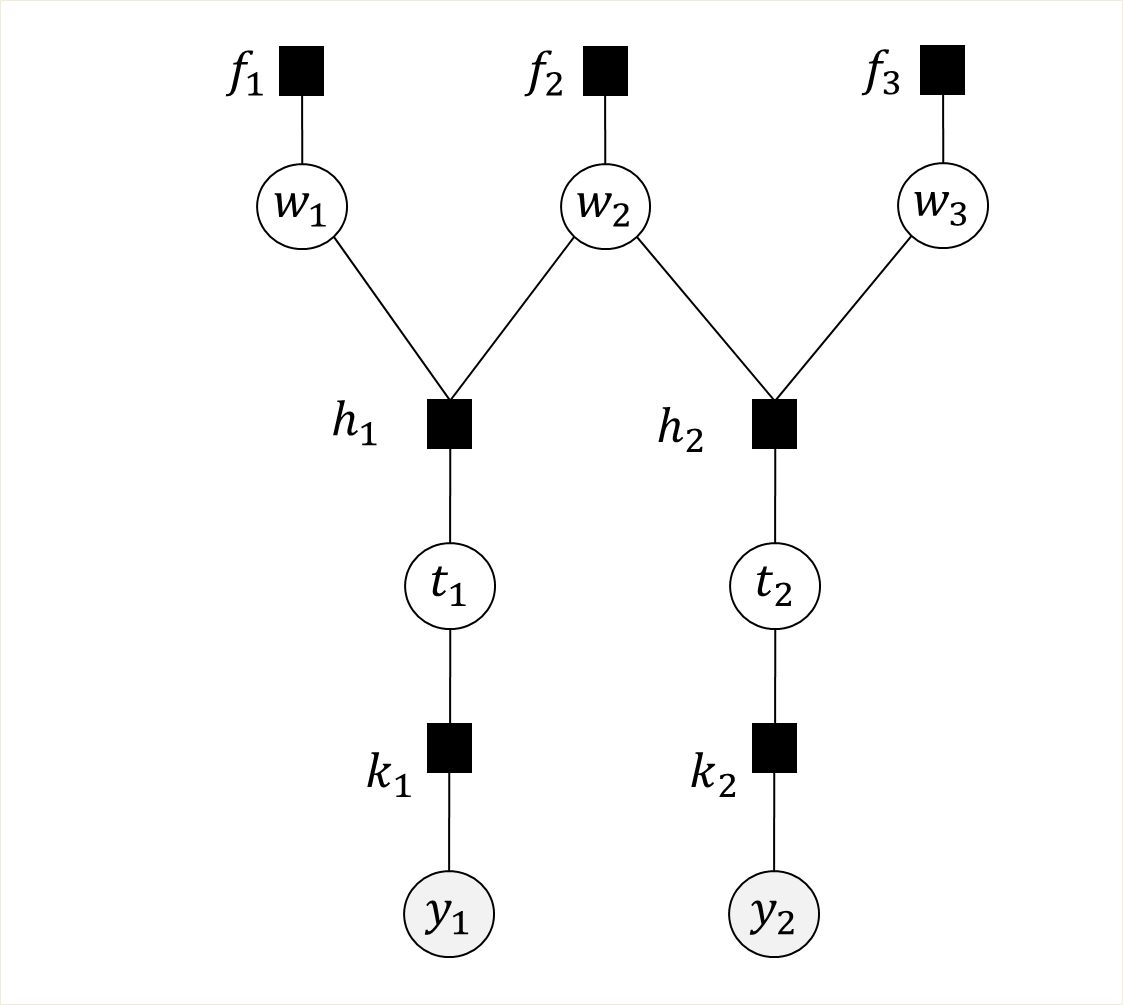
\includegraphics[trim=3cm 0cm 1cm 0cm, clip=true, width=0.4\textwidth]{TrueSkillFullEP1}
}
\parbox{0.59\textwidth}{
Prior factors: $f_i(w_i)=\N(w_i; \mu_0, \sigma_0^2)$\\

``Game'' factors: 
\[
h_g(w_{I_g},w_{J_g},t_g)=\N(t_g; w_{I_g}-w_{J_g},1)
\]
\hfill($I_g$ and $J_g$ are the players in game $g$)\\

Outcome factors:
\[
k_g(t_g, y_g) = \delta\big(y_g - \operatorname{sign}(t_g)\big)
\]

}

We are interested in the marginal distributions of the skills $w_i$.
\begin{itemize}
\item What shape do these distributions have?
\item We need to make some approximations.
\item We will also pretend the structure is a tree (ignore loops).
\end{itemize}

\end{frame}


\begin{frame}
\frametitle{Expectation Propagation in the full TrueSkill graph}

\parbox{0.55\textwidth}{
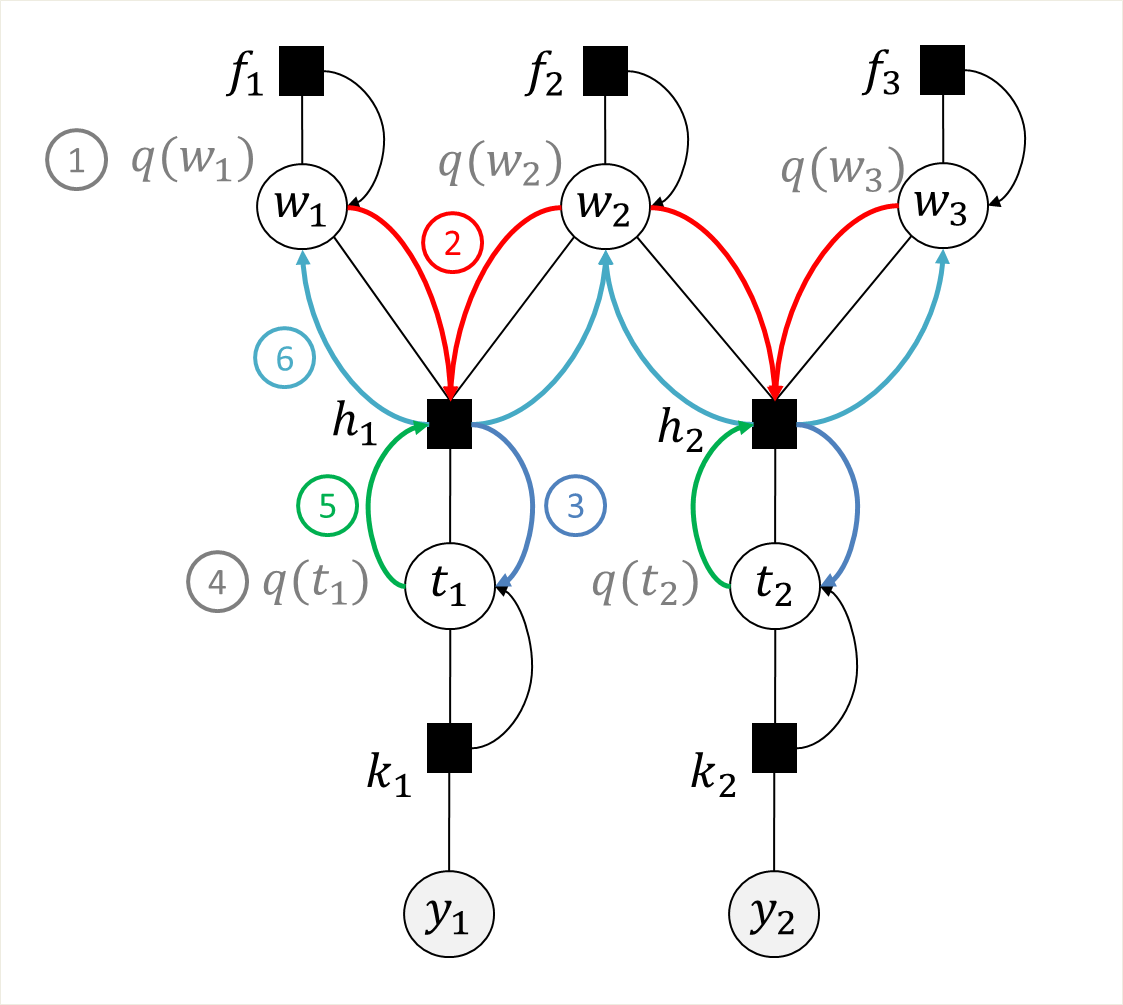
\includegraphics[trim=0.7cm 0.1cm 0.1cm 0.8cm, clip=true, width=0.57\textwidth]{TrueSkillFullEP2}
}
\parbox{0.44\textwidth}{\footnotesize
Iterate\\

(1) Update skill marginals.\\

\Red{(2) Compute skill to game messages.}\\

\Blue{(3) Compute game to performance messages.}\\

(4) Approximate performance marginals.\\

\Green{(5) Compute performance to game messages.}\\

\Cyan{(6) Compute game to skill messages.}
}
\end{frame}


\begin{frame}
\frametitle{Message passing for TrueSkill}

\[
\begin{split}
\Cyan{m^{\tau=0}_{h_g\rightarrow w_{I_g}}\!(w_{I_g})}\;&=\;1,\;\;\;\;
\Cyan{m^{\tau=0}_{h_g\rightarrow w_{J_g}}\!(w_{J_g})}\;=\;1,\;\;\;\;\forall\;g,\\
q^\tau(w_i)\;&=\;f(w_i)\prod_{g=1}^N \Cyan{m^\tau_{h_g\rightarrow w_i}\!(w_i)}
\;\sim\;\N(\mu_i,\sigma^2_i),\\
\Red{m^\tau_{w_{I_g}\rightarrow h_g}\!(w_{I_g})}\;&=\;
\frac{q^\tau(w_{I_g})}{\Cyan{m^\tau_{h_g\rightarrow w_{I_g}}\!(w_{I_g})}},\;\;\;\;
\Red{m^\tau_{w_{J_g}\rightarrow h_g}\!(w_{J_g})}\;=\;
\frac{q^\tau(w_{J_g})}{\Cyan{m^\tau_{h_g\rightarrow w_{J_g}}\!(w_{J_g})}},\\
\Blue{m^\tau_{h_g\rightarrow t_g}\!(t_g)}\;&=\;
\int\!\int h_g(t_g,w_{I_g},w_{J_g}) \Red{m^\tau_{w_{I_g}\rightarrow h_g}\!(w_{I_g})}
\Red{m^\tau_{w_{J_g}\rightarrow h_g}\!(w_{J_g})}dw_{I_g}dw_{J_g},\\
q^{\tau+1}(t_g)\;&=\;{\rm Approx}
\big(\Blue{m^\tau_{h_g\rightarrow t_g}\!(t_g)}m_{k_g\rightarrow t_g}\!(t_g)\big),\\
\Green{m^{\tau+1}_{t_g\rightarrow h_g}\!(t_g)}\;&=\;
\frac{q^{\tau+1}(t_g)}{\Blue{m^\tau_{h_g\rightarrow t_g}\!(t_g)}},\\
\Cyan{m^{\tau+1}_{h_g\rightarrow w_{I_g}}\!(w_{I_g})}\;&=\;\int\!\int
h_g(t_g,w_{I_g},w_{J_g})\Green{m^{\tau+1}_{t_g\rightarrow h_g}\!(t_g)}
\Red{m^\tau_{w_{J_g}\rightarrow h_g}\!(w_{J_g})}dt_gdw_{J_g},\\
\Cyan{m^{\tau+1}_{h_g\rightarrow w_{J_g}}\!(w_{J_g})}\;&=\;\int\!\int
h_g(t_g,w_{J_g},w_{J_g})\Green{m^{\tau+1}_{t_g\rightarrow h_g}\!(t_g)}
\Red{m^\tau_{w_{I_g}\rightarrow h_g}\!(w_{I_g})}dt_gdw_{I_g}.
\end{split}
\]
\end{frame}


\begin{frame}
\frametitle{In a little more detail}

At iteration $\tau$ messages $m$ and marginals $q$ are Gaussian,
with \emph{means} $\mu$, \emph{standard deviations} $\sigma$, \emph{variances}
$v=\sigma^2$, \emph{precisions} $r=v^{-1}$ and \emph{natural means} $\lambda=r\mu$.

\underline{{\bf Step 0} Initialise incoming skill messages:}
\[
\left.\begin{array}{rl} 
\Cyan{r^{\tau=0}_{h_g\rightarrow w_i}}&=\;0\\
\Cyan{\mu^{\tau=0}_{h_g\rightarrow w_i}}&=\;0
\end{array}\!\right\} \Cyan{m^{\tau=0}_{h_g\rightarrow w_i}(w_i)}
\]
\underline{{\bf Step 1} Compute marginal skills:}
\[
\left.\begin{array}{rl} 
r^\tau_i\!\!&=\;r_0+\sum_g \Cyan{r^\tau_{h_g\rightarrow w_i}}\\
\lambda^\tau_i\!\!&=\;\lambda_0+\sum_g \Cyan{\lambda^\tau_{h_g\rightarrow w_i}}
\end{array}\!\right\} q^\tau(w_i)
\]
\underline{{\bf Step 2} Compute skill to game messages:}
\[
\left.\begin{array}{rl}
\Red{r^\tau_{w_i\rightarrow h_g}}\!\!&=\;r^\tau_i-\Cyan{r^\tau_{h_g\rightarrow w_i}}\\
\Red{\lambda^\tau_{w_i\rightarrow h_g}}\!\!&=\;\lambda^\tau_i-\Cyan{\lambda^\tau_{h_g\rightarrow w_i}}
\end{array}\!\right\} \Red{m^\tau_{w_i\rightarrow h_g}\!(w_i)}
\]
\end{frame}


\begin{frame}
\underline{{\bf Step 3} Game to performance messages:}
\[
\left.\begin{array}{rl}
\Blue{v^\tau_{h_g\rightarrow t_g}}\!\!&=\;
1+\Red{v^\tau_{w_{I_g}\rightarrow h_g}}+\Red{v^\tau_{w_{J_g}\rightarrow h_g}}\\
\Blue{\mu^\tau_{h_g\rightarrow t_g}}\!\!&=\;
\Red{\mu^\tau_{I_g\rightarrow h_g}}-\Red{\mu^\tau_{J_g\rightarrow h_g}}
\end{array}\!\right\} \Blue{m^\tau_{h_g\rightarrow t_g}\!(t_g)}
\]
\underline{{\bf Step 4} Compute marginal performances:}
\[
\begin{split}
p(t_g)\;&\propto\;\N(\Blue{\mu^\tau_{h_g\rightarrow
  t_g}},\Blue{v^\tau_{h_g\rightarrow t_g}}){\mathbb
  I}\big(y-\operatorname{sign}(t)\big)\\
&\simeq\;\N(\tilde\mu^{\tau+1}_g, \tilde v^{\tau+1}_g)\;=\;q^{\tau+1}(t_g)
\end{split}
\]
We find the parameters of $q$ by \Blue{\emph{moment matching}}
\[
\left.\begin{array}{rl}
\tilde v^{\tau+1}_g\!\!&=\;\Blue{v^\tau_{h_g\rightarrow t_g}}
\big(1-\Lambda\big(\frac{\Blue{\mu^\tau_{h_g\rightarrow
      t_g}}}{\Blue{\sigma^\tau_{h_g\rightarrow t_g}}}\big)\big)\\
\tilde\mu^{\tau+1}_g\!\!&=\;\Blue{\mu^\tau_{h_g\rightarrow t_g}}+\Blue{\sigma^\tau_{h_g\rightarrow t_g}}
\Psi\big(\frac{\Blue{\mu^\tau_{h_g\rightarrow  t_g}}}{\Blue{\sigma^\tau_{h_g\rightarrow t_g}}}\big)
\end{array}\!\right\}q^{\tau+1}(t_g)
\]
where we have defined $\Psi(x)=\N(x)/\Phi(x)$ and $\Lambda(x)=\Psi(x)(\Psi(x)+x)$.
\end{frame}


\begin{frame}
\underline{{\bf Step 5} Performance to game message:}
\[
\left.\begin{array}{rl}
\Green{r^{\tau+1}_{t_g\rightarrow h_g}}\!\!&=\;\tilde r^{\tau+1}_g -
\Blue{r^\tau_{h_g\rightarrow t_g}}\\
\Green{\lambda^{\tau+1}_{t_g\rightarrow h_g}}\!\!&=\;\tilde\lambda^{\tau+1}_g-
\Blue{\lambda^\tau_{h_g\rightarrow t_g}}
\end{array}\!\right\} \Green{m^{\tau+1}_{t_g\rightarrow h_g}\!(t_g)}
\]
\underline{{\bf Step 6} Game to skill message:}\\
For player 1 (the winner):
\[
\left.\begin{array}{rl}
\Cyan{v^{\tau+1}_{h_g\rightarrow w_{I_g}}}\!\!&=\;1+\Green{v^{\tau+1}_{t_g\rightarrow h_g}}+\Red{v^\tau_{w_{J_g}\rightarrow h_g}}\\
\Cyan{\mu^{\tau+1}_{h_g\rightarrow
 w_{I_g}}}\!\!&=\;\Red{\mu^\tau_{w_{J_g}\rightarrow h_g}}+\Green{\mu^{\tau+1}_{t_g\rightarrow h_g}}
\end{array}\!\right\} \Cyan{m^{\tau+1}_{h_g\rightarrow w_{I_g}}\!(w_{I_g})}
\]
and for player 2 (the looser):
\[
\left.\begin{array}{rl}
\Cyan{v^{\tau+1}_{h_g\rightarrow
  w_{J_g}}}\!\!&=\;1+\Green{v^{\tau+1}_{t_g\rightarrow h_g}}+\Red{v^\tau_{w_{I_g}\rightarrow h_g}}\\
\Cyan{\mu^{\tau+1}_{h_g\rightarrow
 w_{J_g}}}\!\!&=\;\Red{\mu^\tau_{w_{I_g}\rightarrow h_g}}-\Green{\mu^{\tau+1}_{t_g\rightarrow h_g}}
\end{array}\!\right\} \Cyan{m^{\tau+1}_{h_g\rightarrow w_{J_g}}\!(w_{J_g})}
\]
Go back to {\bf Step 1} with $\tau:=\tau+1$ (or stop).
\end{frame}

\end{document}
